\chapter{EEG Mismatch negativity data\label{Chap:data:mmn}}

This chapter describes the analysis of a 128-channel single subject EEG data set acquired from a study of mismatch negativity in the auditory system \cite{marta_mmndcm}. We thank Marta Garrido for providing us with these data. The experiment comprised an auditory oddball paradigm in which subjects heard standard (500Hz) and deviant (550Hz) tones, occuring 80\% (480 trials) and 20\% (120 trials) of the time, respectively, in a pseudo-random sequence subject to the constraint that two deviant tones did not occur together.

EEG data were recorded with a Biosemi\footnote{BioSemi: \url{http://www.biosemi.com/}} system at 128 scalp electrodes and a sampling rate of 512Hz. Vertical and horizontal eye movements were monitored using EOG electrodes. See \cite{marta_mmndcm} for full details of experimental stimuli and recording. To proceed with the data analysis, first download the  data set from the SPM website\footnote{EEG MMN dataset: \url{http://www.fil.ion.ucl.ac.uk/spm/data/eeg\_mmn/}}. The data comprises a file called \texttt{subject1.bdf} whose size is roughly 200MB. We will refer to the directory in which you have placed it as \texttt{DATA\_DIR}. This chapter takes you through different stages of analysis:

\begin{itemize}
\item{Preprocessing}
\item{Sensor space analysis}
\item{Source reconstruction}
\item{Dynamic Causal Modelling}
\end{itemize}

\section{Preprocessing}

There is also an example \matlab\ script under \texttt{man$\backslash$example\_scripts$\backslash$history\_subject1.m} in the SPM distribution which repeats the preprocessing route we take here.

\subsection{Convert}

At the \matlab\ prompt type \texttt{spm eeg}, press the \textsc{Convert} button and select the \texttt{subject1.bdf} file. At the prompt ``Define settings ?'' select ``just read''.

SPM will now read the original Biosemi format file and create an SPM compatible data file, called \texttt{spm8\_subject1.mat} and \texttt{spm8\_subject1.dat} in the directory containing the original data file (\texttt{DATA\_DIR}).

\subsection{Montage}

In this step, we will identify the VEOG and HEOG channels, and also remove several channels that don't carry EEG data and are of no importance to the following. In this case we apply montage as the first processing step to set all the channel types correctly for subsequent processing. This is especially important for the EOG channels, which are derived from channels that would not normally be filtered because SPM does not recognize them as containing M/EEG data. We generally recommend to remove all data channels that are no longer needed because it will reduce the total file size. We will also convert the data to average reference montage by subtracting from each channel the mean of all EEG channels. To do so, we use the \textsc{montage} tool in SPM, which is a general approach for pre-multiplying the data matrix (channels $\times$ time) by another matrix that linearly weights all channel data. This provides a very general method for data transformation in M/EEG analysis.

The appropriate montage-matrix can be derived as follows.
In our case, we would like to only keep EEG channels 1 to 128 and subtract from each channel the average of all EEG channels. In addition, there were three EOG channels (129, 130, 131), where the HEOG is computed as the difference between channels 131 and 130, and the VEOG by the difference between channels 130 and 129. This matrix can be specified in SPM by either using a graphical interface, or by supplying the matrix saved in a file. We will do the latter. The script to generate this file can be found in the \texttt{example\_scripts} folder: \texttt{montage\_subject1.m}. Copy this script into \texttt{DATA\_DIR} and run it. This will generate a file named \texttt{MONT\_EXP.mat}.

You now call the montage function by choosing \textsc{Montage} in the ``Other'' drop-down menu and:
\begin{itemize}
\item{Select the M/EEG-file \texttt{spm8\_subject1.mat}}
\item{`How to specify the montage ?' Answer ``file''.}
\item{Then select the generated \texttt{MONT\_EXP.mat} file}
\item{``Keep the other channels?'' : ``No''}
\end{itemize}
This will remove the uninteresting channels from the data. The progress bar appears and SPM will generate two new files \texttt{Mspm8\_subject1.mat} and \texttt{Mspm8\_subject1.dat}.

This step will also assign default locations to the sensors, as this information is not contained in the original Biosemi \texttt{*.bdf} file. It is usually the responsibility of the user to link the data to sensors which are located in a coordinate system. In our experience this is a critical step. SPM provide tools (\textsc{Prepare}) for linking data and location information, leaving it the responsibility of the user to verify the success of this process. Chapter \ref{Chap:eeg:preprocessing} describes in detail how you can use the \textsc{Prepare} tool from the ``Other'' drop-down menu to use digitized sensor location data.


\subsection{Filter}
Filtering the data in time removes unwanted frequency bands from the data. Usually, for evoked response analysis, the low frequencies are kept, while the high frequencies are assumed to carry noise. Here, we will use a highpass filter to remove ultra-low frequencies close to DC, and a lowpass filter to remove high frequencies. We filter prior to downsampling because otherwise high-amplitude baseline shifts present in the data will generate filtering artefacts at the edges of the file. 
\begin{itemize}
\item{Click on \textsc{Filter} and select the \texttt{Mspm8\_subject1.mat} file.}
\item{Select a ``highpass'' filter with cutoff of 0.5 (Hz).}
\end{itemize}
The progress bar will appear and the resulting filtered data will be saved in files \texttt{fMspm8\_subject1.mat} and \texttt{fMspm8\_subject1.dat}. 
\begin{itemize}
\item{Click on \textsc{Filter} and select the \texttt{fMspm8\_subject1.mat} file.}
\item{Select a ``lowpass'' filter with cutoff of 30 (Hz).}
\end{itemize}
The progress bar will appear and the resulting filtered data will be saved in files \texttt{ffMspm8\_subject1.mat} and \texttt{ffMspm8\_subject1.dat}. 

\subsection{Downsample}
Here, we will downsample the data in time. This is useful when the data were acquired like ours with a high sampling rate of 512 Hz. This is an unnecessarily high sampling rate for a simple evoked response analysis, and we will now decrease the sampling rate to 200 Hz, thereby reducing the file size by more than half. Select \textsc{Downsample} from the ``Other'' drop-down menu and select the \texttt{ffMspm8\_subject1.mat} file. Choose a new sampling rate of 200 (Hz). The progress bar will appear and the resulting data will be saved to files \texttt{dffMspm8\_subject1.mat} and \texttt{dffMspm8\_subject1.dat}. This step requires the Signal Processing Toolbox.

\subsection{Epoch}
To epoch the data click on \textsc{Epoching}. Select the \texttt{dffMspm8\_subject1.mat} file. Choose the peri-stimulus time window, first the start \texttt{-100}, then the end \texttt{400} ms. Choose 2 conditions. You can call the first condition ``standard''. A GUI pops up which gives you a complete list of all events in the EEG file. The standard condition had 480 trials, so select the type with value 1 and press OK. The second condition can be called ``rare''. The rare stimulus was given 120 times and has value 3 in the list. Select this trial type and press OK. Answer two times ``no'' to the questions  ``review individual trials'', and ``save trial definitions''. The progress bar will appear and the epoched data will be saved to files \texttt{edffMspm8\_subject1.mat} and \texttt{edffMspm8\_subject1.dat}.
\begin{figure}
\begin{center}
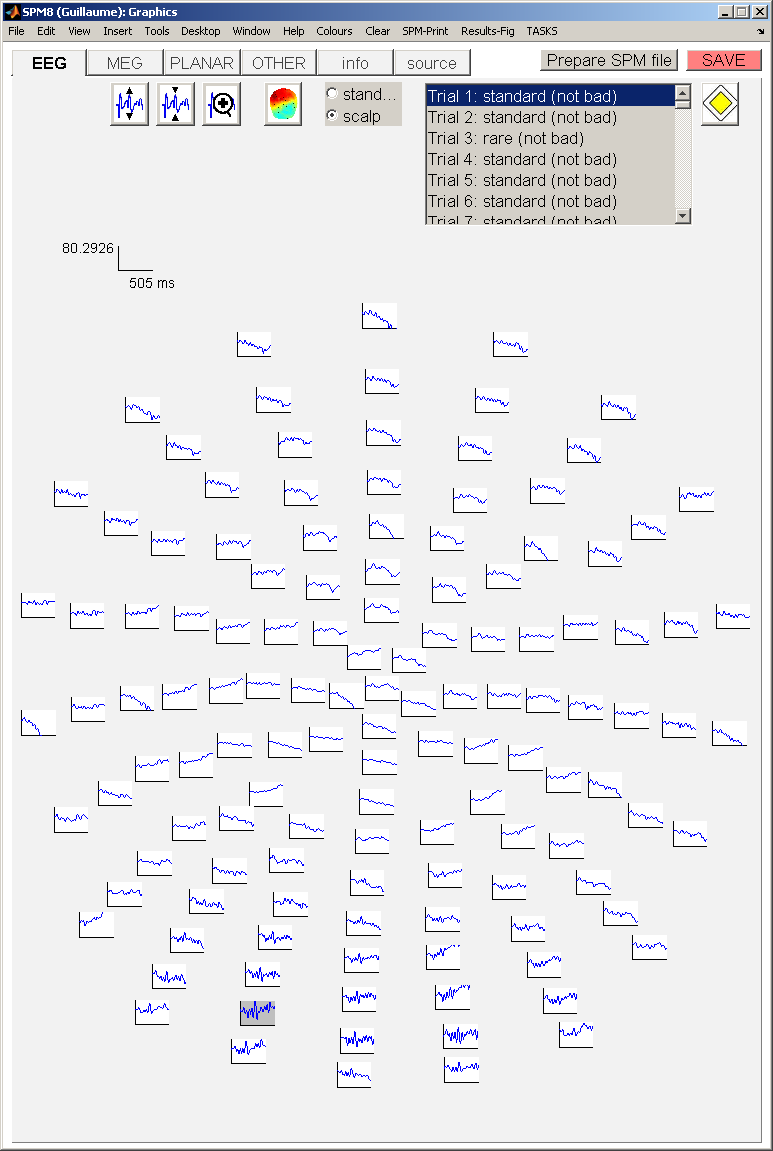
\includegraphics[width=150mm]{mmn/topo1}
\caption{\em Scalp topography of single trial MMN EEG data. Channel 14, second-row from bottom, left hemisphere contains (slightly) higher variability data than the others. This channel is to be marked as artefactual (ie. 'bad').
\label{topo1}}
\end{center}
\end{figure}

\subsection{Artefacts}
 A number of different methods of artefact removal are implemented in SPM8. Here, we will demonstrate a simple thresholding method. However, before doing so, we will look at the data in the display:
\begin{itemize}
\item{Choose ``M/EEG'' from the ``Display'' dropdown menu.}
\item{Select the \texttt{edffMspm8\_subject1.mat} file.}
\item{Click on the ``EEG'' tab.}
\item{Press the ``scalp'' radio button.}
\end{itemize}
The time-series for the first trial will then appear in the topographical layout shown in Figure~\ref{topo1}.

 You will see that Channel 14, second-row from bottom, left hemisphere, contains (slightly) higher variability data than the others .
Right-click on the channel; this tells you that this channel is ``A14''. You will also see as an entry in this menu ``bad: 0''. Select this entry, and click the left button. This will make the menu disappear, but the channel now has a grey background. You have marked this channel as bad. Click on ``save''in the top-right corner. This channel will then be ignored in subsequent processing. In fact this channel probably doesn't need removing, but we do so for teaching purposes only.
\\
\\
Now, click on \textsc{Artefacts}. A window of SPM8 batch interface will open. You might be already familiar with this interface from other SPM8 functions. It is also possible to use the batch interface to run the preprocessing steps that we have performed until now, but for artefact detection this is the only graphical interface. Click on ``File name'' and select the \texttt{edffMspm8\_subject1.mat} file.  Double click ``How to look for artefacts'' and a new branch will appear. It is possible to define several sets of channels to scan and several different methods for artefact detection. We will use simple thresholding applied to all channels. Click on ``Detection algorithm'' and select ``Threshold channels'' in the small window below. Double click on ``Threshold'' and enter 80 (in this case $\mu V$). The batch is now fully configured. Run it by pressing the green button at the top of the batch window. 

This will detect trials in which the signal recorded at any of the channels exceeds 80 microvolts (relative to pre-stimulus baseline). These trials will be marked as artefacts. Most of these artefacts occur on the VEOG channel, and reflect blinks during the critical time window. The procedure will also detect channels in which there are a large number of artefacts (which may reflect problems specific to those electrodes, allowing them to be removed from subsequent analyses).

In this case, the Matlab window will show:
\begin{verbatim}
1 bad channels: A14 
77 rejected trials:  3    4    5    7    8    9   10   12   28   29   88  [...]
Done    'M/EEG Artefact detection'
Done
\end{verbatim}
A new file will also be created, \texttt{aedffMspm8\_subject1.mat}.

There are also interactive artefact removal routines available from \texttt{Toolbox} $\rightarrow$ \texttt{MEEG tools} $\rightarrow$  \texttt{Fieldtrip visual artifact rejection}.

\subsection{Averaging}
To produce an ERP click on \textsc{Averaging} and select the \texttt{aedffMspm8\_subject1.mat} file. At this point you can perform either ordinary averaging or ``robust averaging''. Robust averaging makes it possible to supress artefacts automatically without rejecting trials or channels compltely, but just the contaminated parts. For robust averaging answer ``yes'' to `Use robust averaging?''. Answer ``yes'' to ``Save weights'', and ``yes'' to ``Compute weights by condition'' \footnote{In this case we do not want to pool both conditions together because the number of standard and rare trials are quite different.} and press ``Enter'' to accept the default ``Offset of the weighting function''. A new dataset will be generated \texttt{maedffMspm8\_subject1}  and automatically opened in the reviewing tool so that you can examine the ERP. There will also be an additional dataset named \texttt{WaedffMspm8\_subject1} this dataset will contain instead of EEG data the weights used by robust averaging. This is useful to see what was suppressed and whether there might be some condition-specific bias that could affect the results.

The Graphics window will pop up and allow you to look at the averaged data. To look at the ERP, click on the EEG tab, and press the ``scalp'' radio button. Now hold  the Shift button down on the keyboard whilst selecting trial 2 with the left mouse button in the upper right corner of the graphics window. This will overlay responses to standard and rare trials on the same figure axes.

Now press the ``plus'' icon at the top of this graphics window and select channel C23 (seventh central channel down from the top) with a left mouse click. This will plot the ERPs shown in Figure~\ref{c23}. This completes the preprocessing step.
\begin{figure}
\begin{center}
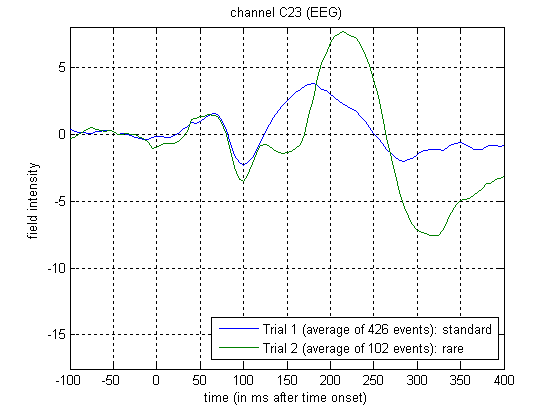
\includegraphics[width=120mm]{mmn/erp_c23}
\caption{\em ERPs at channel C23 (CZ) for standard and rare tones. The ERP curve for rare tones lies underneath that for standard tones between 100 and 180ms. This corresponds to the mismatch negativity signal in this subject. \label{c23}}
\end{center}
\end{figure}

\subsection{History}
The evoked response file (and every other SPM MEEG data file) contains a history-entry which stores all of the above preprocessing steps. You can take this history and produce a script that will re-run the same analysis which you entered using the GUI. See the ``history'' tab in the ``info'' section when displaying the data. Chapter \ref{Chap:eeg:preprocessing} provides more details on this.

\section{Sensor space analysis}

A useful feature of SPM is the ability to use Random Field Theory to correct for multiple statistical comparisons across N-dimensional spaces. For example, a 2D space representing the scalp data can be constructed by flattening the sensor locations and interpolating between them to create an image of MxM pixels (when M is user-specified, eg M=32). This would allow one to identify locations where, for example, the ERP amplitude in two conditions at a given timepoint differed reliably across subjects, having corrected for the multiple t-tests performed across pixels. That correction uses Random Field Theory, which takes into account the spatial correlation across pixels (i.e, that the tests are not independent). 
Here, we will consider a 3D example, where the third dimension is time, and test across trials within this single subject. We first create a 3D image for each trial of the two types, with dimensions M$\times$M$\times$S, where S=101 is the number of samples (time points). We then take these images into an unpaired t-test across trials (in a 2nd-level model) to compare ``standard'' and ``rare'' events. We can then use classical SPM to identify locations in space and time in which a reliable difference occurs, correcting across the multiple comparisons entailed. This would be appropriate if, for example, we had no a priori knowledge where or when the difference between standard and rare trials would emerge. The appropriate images are created as follows
\begin{itemize}
\item{Select the ``Convert to image'' option from the ``Other'' pulldown menu.}
\item{Select the \texttt{aedffMspm8\_subject1.mat} file.}
\item{For ``output image dimensions'' accept the default of 32 (leading to a 32x32 pixel space).}
\item{For ``interpolate' or ``mask out'' bad channels, select ``interpolate''.}
\end{itemize}
SPM will take some time as it writes out a NIfTI image for each trial (except rejected trials), in a new directory called \texttt{aedffMspm8\_subject1}, which will itself contain two subdirectories, one for each trialtype, called \texttt{type\_rare} and \texttt{type\_standard}. In each trialtype subdirectory there will be image and header files for each non-rejected trial of that type, e.g, trial0001.img/hdr. You can press ``Display: images'' to view one of these images - it will have dimensions 32$\times$32$\times$101.

To perform statistics on these images:
\begin{itemize}
\item{Create a new directory, eg. \texttt{mkdir XYTstats}.}
\item{Press the ``Specify 2nd level'' button.}
\item{Select ``two-sample t-test'' (unpaired t-test)}
\item{Define the images for ``Group 1'' as all those in the subdirectory \texttt{type\_standard} (using right mouse, and ``select all'') and the images for ``Group 2'' as all those in the subdirectory \texttt{type\_rare}.}
\item{Finally, specify the new \texttt{XYTstats} directory as the output directory.}
\item{Press the ``save'' icon, top left, and save this design specification as \texttt{mmn\_design.mat} and press ``save''.}
\item{Press the green ``Run'' button to execute the job\footnote{Note that we can use the default ``nonsphericity'' selections, i.e, that the two trial-types may have different variances, but are uncorrelated.} This will produce the design matrix for a two-sample t-test.} 
\item{Now press ``Estimate'' in SPMs main window, and select the \texttt{SPM.mat} file from the \texttt{XYTstats} directory.}
\end{itemize}
Now press ``Results'' and define a new F-contrast as [1 -1] (for help with these basic SPM functions, see eg. chapter~\ref{Chap:data:auditory}). Keep the default contrast options, but threshold at $p<.05$ FWE corrected for the whole search volume and select ``Scalp-Time'' for the ``Data Type''. Then press ``whole brain'', and the Graphics window should now look like that in Figure~\ref{3DSPM}. This reveals a large fronto-central region within the 2D sensor space and within the time epoch in which standard and rare trials differ reliably, having corrected for multiple F-tests across pixels/time. An F-test is used because the sign of the difference reflects the polarity of the ERP difference, which is not of primary interest.
 
The cursor in Figure~\ref{3DSPM} has been positioned by selecting the second cluster in the results table. This occurs at time point 160ms post stimulus.
 
 \begin{figure}
\begin{center}
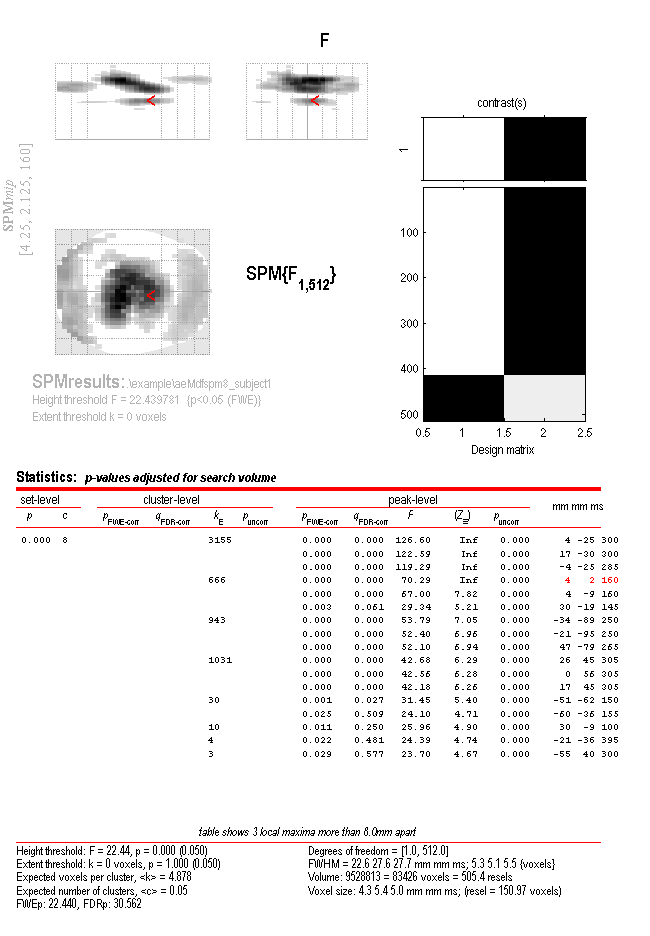
\includegraphics[width=120mm]{mmn/3DSPM}
\caption{\em In this SPM the time axis is reflected in the two MIP windows in the top row, with time proceeding from the bottom to the top of the page. The cursor has been positioned by selecting the third cluster in the results table. This occurs at time point 160ms post stimulus. The design matrix on the right hand side comprises two columns, the first for standard trials and the second for rare ones. \label{3DSPM}}
\end{center}
\end{figure}
Now:
\begin{itemize}
\item{Press the right mouse button in the MIP}
\item{Select ``display/hide channels''}
\item{Select the \texttt{maedffMspm8\_subject1.mat} file.}
\end{itemize}
This links the \texttt{SPM.mat} file with the M/EEG file from which the EEG images were created.
It is now possible to superimpose the channel labels onto the spatial SPM, and also to ``goto the nearest channel'' (using options provided after a right mouse click, when navigating the MIP).
 
We have demonstrated sensor space analysis for single-subject data. More frequently, one would compute ERP images for each subject, smooth them, and then perform paired t-tests over subjects to look for condition differences. See \cite{marta_mmndcm} for a group analysis of MMN data.
 
Finally, if one had more constrained a priori knowledge about where and when the differences would appear, one could perform a Small Volume Correction (SVC) based on, for example, a box around fronto-central channels and between 100 and 200ms poststimulus. We also refer the reader to chapter \ref{Chap:eeg:sensoranalysis} for further details on sensor space analysis.

\section{Source reconstruction}

Source reconstruction comprises forward modeling and inverse modeling steps and is implemented by pressing the 3D source reconstruction button in SPM's top-left window.
This brings up the source localisation GUI shown in Figure~\ref{source_gui}. The following subsections detail each of the steps in a source reconstruction analysis. We also advise the reader to consult the reference material in chapter \ref{Chap:eeg:imaging}.

\begin{figure}
\begin{center}
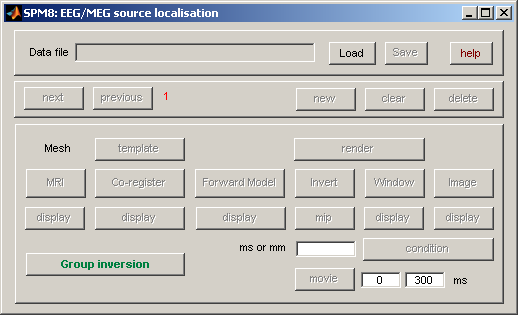
\includegraphics[width=120mm]{mmn/source_gui}
\caption{\em Graphical user interface for 3D source localisation. A complete localisation comprises the following steps (i) creation of a cortical mesh, (ii) co-registration of the mesh with M/EEG data, (iii) creation of a forward model, and (iv) results interrogation. As each of these steps is completed the relevant part of the GUI becomes highlighted (text appears more solid).
\label{source_gui}}
\end{center}
\end{figure}

\subsection{Mesh}
The first step is to load the data and create a cortical mesh upon which M/EEG data will be projected:
\begin{itemize}
\item{Press the ``Load'' button in the souce localisation GUI and select the file \texttt{maedffMspm8\_subject1.mat}.}
\item{Enter ``Standard'' under ``Comment/Label for this analysis'' and press OK.}
\item{Now press the ``template'' button.}
\item{For ``Cortical mesh'', select ``normal''.}
\end{itemize}
SPM will then form the ``standard'' or ``canonical'' cortical mesh shown in the Graphics window which, after rotation, should look like Figure~\ref{mesh}
\begin{figure}
\begin{center}
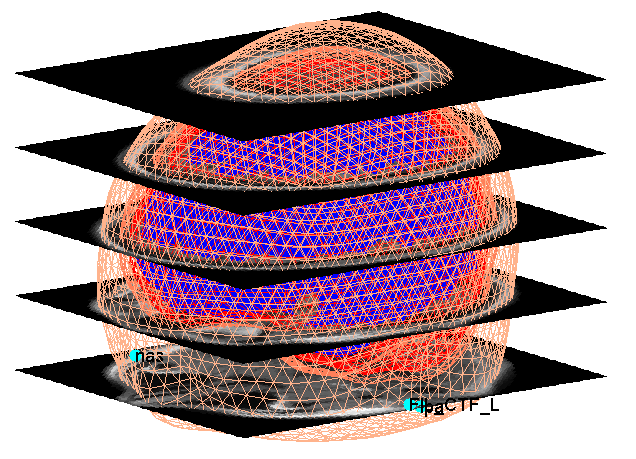
\includegraphics[width=120mm]{mmn/mesh}
\caption{\em The figure shows the canonical cortical mesh (blue), inner skull surface (red) and scalp surface (light brown). The hardwired fiducials are shown in light blue. Transverse slices of canonical MRI are also shown in black, with gray scale inlays showing anatomical detail.
\label{mesh}}
\end{center}
\end{figure}

\subsection{Coregister}

Now press the ``Co-register'' button. This will create further output in the Graphics window, the upper panel of which should like like Figure~\ref{coreg}.
\begin{figure}
\begin{center}
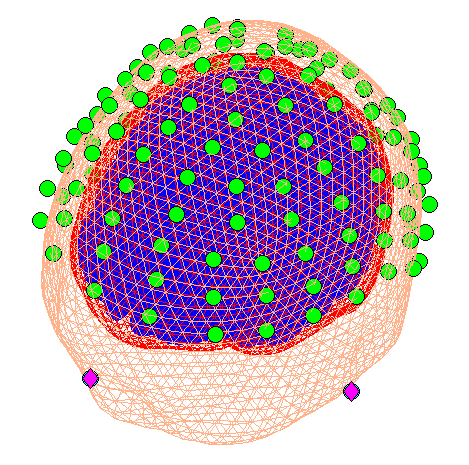
\includegraphics[width=120mm]{mmn/coreg}
\caption{\em
The figure shows the MRI fiducials (pink), the sensor fiducials (blue) and the locations of sensors (green) in addition the the canonical cortical mesh (blue), inner skull surface (red) and scalp surface (light brown).
\label{coreg}}
\end{center}
\end{figure}

In this coregister step we were not required to enter any further parameters. However, if you are not using the template (or ``canonical'' mesh) or if at the ``prepare'' stage above you loaded your own (non-standard) sensor positions then you will be asked for the locations in MNI coordinates of the fiducial positions.

\subsection{Forward model}

Now press the ``Forward model'' button. Then select ``EEG-BEM'' in response to the ``Which EEG head model?'' question. SPM will then use a Boundary Element Method (BEM) which will take approximately 10 minutes to run. Upon completion SPM will write the \texttt{single\_subj\_T1\_EEG\_BEM.mat} file into the canonical subdirectory of your SPM distribution. The Graphics window should now appear as in Figure~\ref{forward}.
\begin{figure}
\begin{center}
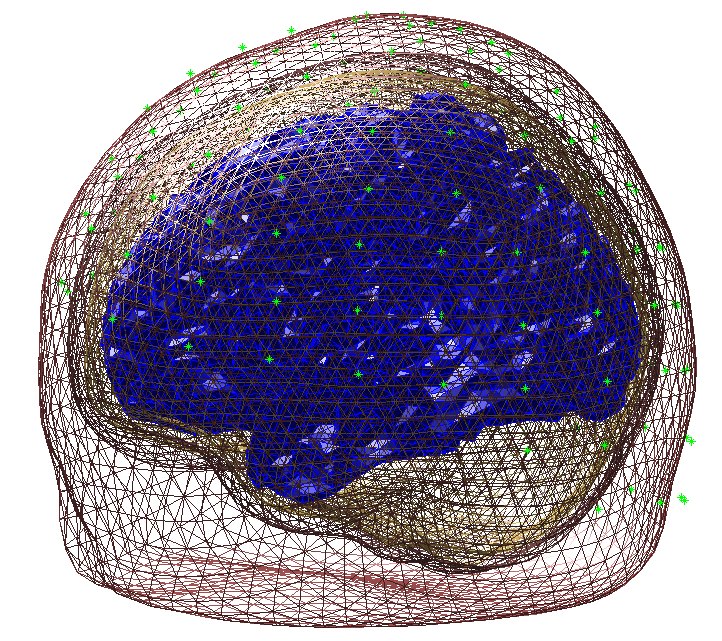
\includegraphics[width=120mm]{mmn/forward}
\caption{\em
The figure shows the cortical mesh (blue), brain, skull and scalp surfaces. Electrode positions are marked with asterisks.
\label{forward}}
\end{center}
\end{figure}
The next time you wish to use an EEG-BEM solution based on the template mesh, SPM will simply use the date from the \texttt{single\_subj\_T1\_EEG\_BEM.mat} file (so this step will be much quicker the next time you do it). The same principle applies to EEG-BEM solutions computed from meshes based on subjects individual MRIs.

\subsection{Invert}

Now press the Invert button and
\begin{itemize}
\item{Select an ``Imaging'' reconstruction.}
\item{Select ``Yes'' for ``All conditions or trials''.}
\item{Select ``Standard'' for Model.}
\end{itemize}
SPM will now compute a leadfield matrix and save it in the file \texttt{SPMgainmatrix\_maedffMspm8\_subject1\_1.mat} placed in \texttt{DATA\_DIR}. This file can be replaced with one computed using other methods for computing the lead field (eg methods external to SPM). The forward model will then be inverted using the Multiple Sparse Priors (MSP) algorithm (the progress of which is outputted to the \matlab\ command window). SPM will produce, in the Graphics window, (i) a Maximum Intensity Projection (MIP) of activity in source space (lower panel) and (ii) a time series of activity for (upper panel) each condition.

The ``ms or mm'' window has three functionalities (i) if you enter a single number this will be interpreted as ms, (ii) if you enter two numbers this will be interpreted as a time window for plotting movies (see below), (iii) if you enter 3 numbers this will be interpreted as MNI coordinates for a time series plot.

Now enter ``160'' for ``ms or mm'' and press the MIP button, to see a MIP of activity in source space at 160ms post-stimulus, and the time series of activities (top panel) at the position with largest magnitude signal. The corresponding graphic is shown in Figure~\ref{invert}. By toggling the ``Condition'' button, and pressing MIP each time, you can view the spatial distribution of activity for the different conditions (at the selected time point).
\begin{figure}
\begin{center}
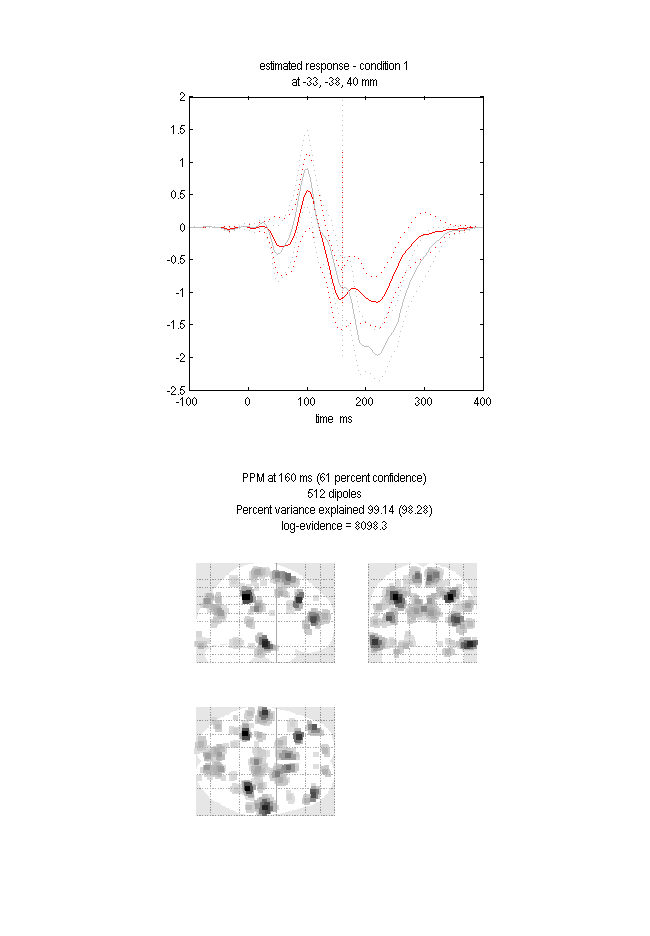
\includegraphics[width=120mm]{mmn/invert}
\caption{\em Source reconstructed activity at 160ms post-stimulus.
The upper trace shows responses to Condition 1 (Standards) with the red curve, and to Condition 2 (Rare) in gray.
\label{invert}}
\end{center}
\end{figure}

\section{Dynamic Causal Modeling}

Many of the functionalities of DCM for M/EEG are described in more detail in the reference chapter \ref{Chap:eeg:DCM}. In this chapter we demonstrate only the ``DCM for ERP'' model. 
Users are strongly encouraged to read the accompanying theoretical papers \cite{od_dcm_erp,sjk_dcm_erp}. Briefly, DCM for ERP fits a  neural network model to M/EEG data, in which activity in source regions are described using differential equations based on neural mass models. Activity in each region comprises three populations of cells; pyramidal, local excitatory and local inhibitory. Fitting the model will then allow you to plot estimated activity in each cell population in each region. It will also provide estimates of the long range connections between regions, and show how these values are changed by experimental manipulation (eg. rare versus standard trial types).
  
In the \texttt{example\_scripts} folder of the SPM distribution, we also provide an example script that will run a DCM-for-ERP analysis of this data. This can be edited to implement your own analysis.

Pressing the ``DCM'' button will open up the DCM GUI shown in Figure~\ref{dcm_gui}.
\begin{figure}
\begin{center}
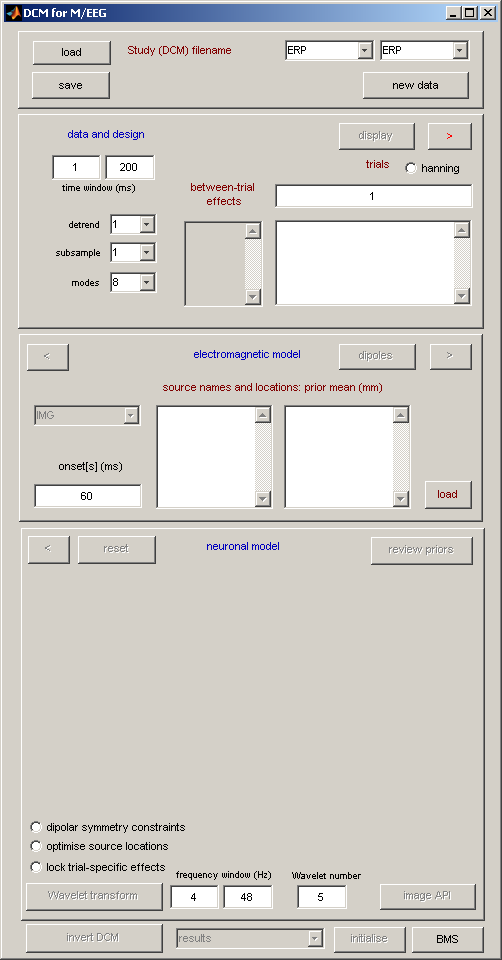
\includegraphics[width=80mm]{mmn/dcm_gui}
\caption{\em The Dynamic Causal Modeling GUI splits model specification into three reversible phases (i) data and design, (ii) electromagnetic model and (iii) neuronal model. One can move forwards and backwards in the model specification using the left and right arrow buttons (these become highlighted when sufficient information has been entered to proceed to the next step).
\label{dcm_gui}}
\end{center}
\end{figure}
\begin{figure}
\begin{center}
%\includegraphics[width=80mm]{mmn/}
(a)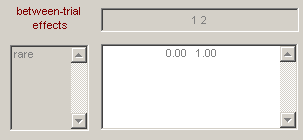
\includegraphics[width=80mm]{mmn/data_and_design}
(b)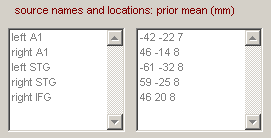
\includegraphics[width=80mm]{mmn/electro_model}
(c)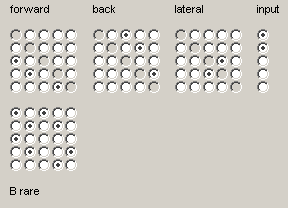
\includegraphics[width=80mm]{mmn/neuronal_model}
\caption{\em Specification of DCM for ERP model (a) Data and design, (b) electromagnetic model and (c) neuronal model.
\label{specify} }
\end{center}
\end{figure}
We will now complete the three model specification entries shown in Figure~\ref{specify}:
\begin{itemize}
\item{Press the ``new data'' button and select the \texttt{maedffMspm8\_subject1.mat} file.}
\item{Enter the ``between-trial effects'' and design matrix information shown in Figure~\ref{specify}(a).}
\item{Press the ``Display'' button.}
\end{itemize}
This completes the data specification stage. Now:
\begin{itemize}
\item{Press the right hand arrow to move on to the specification of the electromagnetic model.}
\item{Instead of ``IMG'' select ''ECD'' for the spatial characteristics of the sources.}
\item{Now enter the names and (prior mean) locations of the sources shown in Figure~\ref{specify}(b).}
\item{Pressing the ``dipoles'' button will create an interactive display in the graphics window showing the prior source positions.}
\end{itemize}
This completes the specification of the electromagnetic model. Now:
\begin{itemize}
\item{Press the right hand arrow (next to the dipoles button) to move on to specification of the neuronal model.}
\item{Highlight the connectivity matrix radio buttons so that they  correspond to those shown in Figure~\ref{specify}(c).}
\item{Press the (top left) 'save' button and accept the default file name.}
\item{Press 'Invert DCM'}
\end{itemize}
SPM will plot the progess of the model estimation in the MATLAB command window. Plots of data and the progressing model fit will be shown in SPM's graphics window. The algorithm should converge after five to ten minutes (in 64 iterations). Now select the ``ERPs (sources)'' option from the pull down menu to the right of the ``Estimated'' button. This will produce the plot shown in Figure~\ref{source_erps}. The values of the connections between areas can be outputted by selecting eg ''Coupling(A)'' from the pull-down menu in the DCM GUI. This will allow you to interrogate the posterior distribution of model parameters. It is also possible to fit multiple models, eg. with different numbers of regions and different structures, and to compare them using Bayesian Model Comparison. This is implemented by pressing the BMS button (bottom right hand corner of the DCM window).

\begin{figure}
\begin{center}
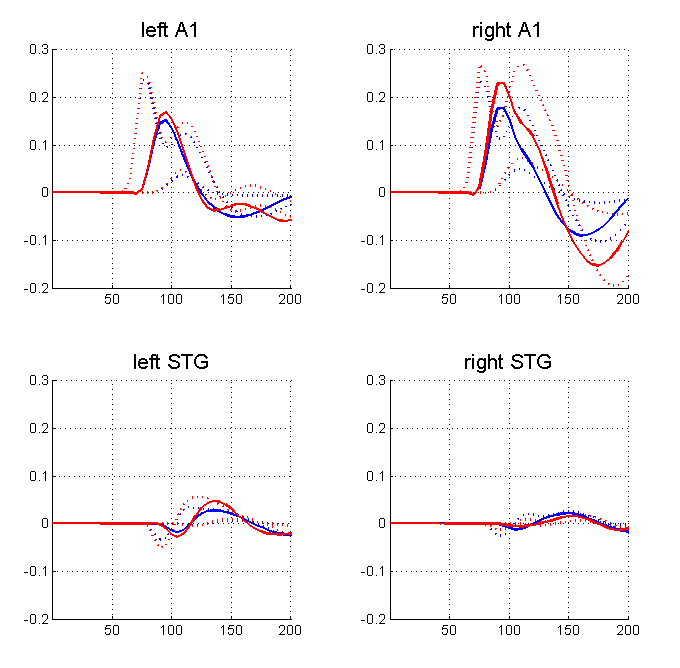
\includegraphics[width=120mm]{mmn/source_erps}
\caption{\em Activity plots for three neuronal populations (solid lines for pyramidal cells, dotted lines for others), in four areas (fifth not shown in this figure), for standard (blue) and rare (red) trial types.
\label{source_erps} }
\end{center}
\end{figure}
